\documentclass[]{article}

\usepackage{lmodern}
\usepackage[T1]{fontenc}
\input{H_structue}
\usepackage[a4paper, margin=1.2in]{geometry}
\definecolor{cover}{RGB}{230, 194, 24}
\begin{document}


%----------------------------------------------------------------------------------------
%	TITLE PAGE
%----------------------------------------------------------------------------------------
\begingroup
\AddToShipoutPicture*{\put(0,0){
\includegraphics[width=\paperwidth,height=\paperheight]{Cover1.jpg}}}
\par\sffamily\selectfont
\color{cover}
\fontsize{80pt}{0}\selectfont Partial\par
\fontsize{80pt}{0}\selectfont Differential\par
\fontsize{80pt}{0}\selectfont Equations\par
\begin{center}
    {\LARGE 01356 Spring 2023}\par
    \vspace*{1cm}
    {\Huge Lecture Notes}\par       
\end{center}
\color{white}
\vspace*{4.5cm}
\fontsize{22pt}{0}\selectfont Lecturer: Prof. Mahmoud M. El-Borai\par
\fontsize{22pt}{0}\selectfont Prepared by: Ossama Abdelwahed And\par
\hspace*{4cm}
\fontsize{22pt}{0}\selectfont Ahmed.M.Habib\par
\endgroup

\newpage

\tableofcontents

\newpage

\section{Introduction}
The main goal of many scientfic displines can be summerized to the following:

\begin{enumerate}
\item Formulate a set of mathematical equations to model a phenomena of intrest
\item Analyze solutions to these equations in order to extract information and make predictions.
\end{enumerate}

The result of 1 is often a system of partial differential equations, thus the second becomes solving those partial differential equations.
\par
A partial differential equation (PDE) is is a differential equation containing partial derivatives of the dependent variable with repect to more than one independent variable.

\subsection{Order of PDE}
The order of a PDE is determined by the highest derivative in the equation.
\begin{align*}
\frac{\partial u}{\partial t} + {(\frac{\partial u}{\partial x})}^2 &= 0 \ \ \ \ \Longrightarrow  \text{First order}
\\
\frac{\partial^4 u}{\partial y^4} + \frac{\partial u}{\partial x} &= c \ \ \ \ \Longrightarrow  \text{Fourth order}
\end{align*}
do not mistake the order of the PDE with its degree, the degree of the PDE is the highest exponent appearing in the equation.
\subsection{Linearity} 
A linear PDE is one that is of first degree in all of its field variables and partial derivatives.
\begin{align*}
\frac{\partial u}{\partial t} + \frac{\partial u}{\partial x} &= 0 \quad\quad \text{linear}
\\
\frac{\partial^4 u}{\partial y^4} + \frac{\partial u}{\partial x} &= y \quad\quad \text{linear}
\\
\frac{\partial u}{\partial t} + {(\frac{\partial u}{\partial x})}^2 &= 0 \quad\quad \text{nonlinear}
\\
\frac{\partial^3 u}{\partial x^3} + {(\frac{\partial^2 u}{\partial y^2})}^5 &= \sin(x) \quad\quad \text{nonlinear}
\end{align*}

a linear operator can be defined for any linear equation, taking the first equation in the previous list, the linear operator $L$ can be defined as.
\[
L = \frac{\partial }{\partial t} + \frac{\partial u}{\partial x}
\]
and the equation can be written as.
\[
    L(u)=0    
\]

\subsection{Homogeneity}
Let $L$ be a linear operator. Then a linear partial differential equation can be written in the form.
\[
    L(u) = f(x_1,x_2, \dots , t)    
\]
if $f = 0$ then the equation is homogeneous, otherwise it is inhomogeneous.
\begin{align*}
\frac{\partial u}{\partial t} + \frac{\partial u}{\partial x} &= 0 \quad\quad \text{homogeneous}
\\
\frac{\partial^4 u}{\partial y^4} + \frac{\partial u}{\partial x} &= y \quad\quad \text{inhomogeneous}
\end{align*}

\subsection{Boundry Conditions}
Boundary conditions are constraints necessary for the solution of a boundary value problem. A boundary value problem is a differential equation to be solved in a domain on whose boundary the function is known. We will be intrested in one type of boundry conditions in this course which is the Drichlet Conditions, specifies the value that the unknown function needs to take on along the boundary of the domain. For example, the Laplace equation on a circle with drichlet condition will be.
\[
    \nabla^2 u(x) = 0 \;\;\;\; \forall x \in G    
\]
\[
    u(x) = f(x) \;\;\;\; \forall x \in G    
\]
\begin{center}
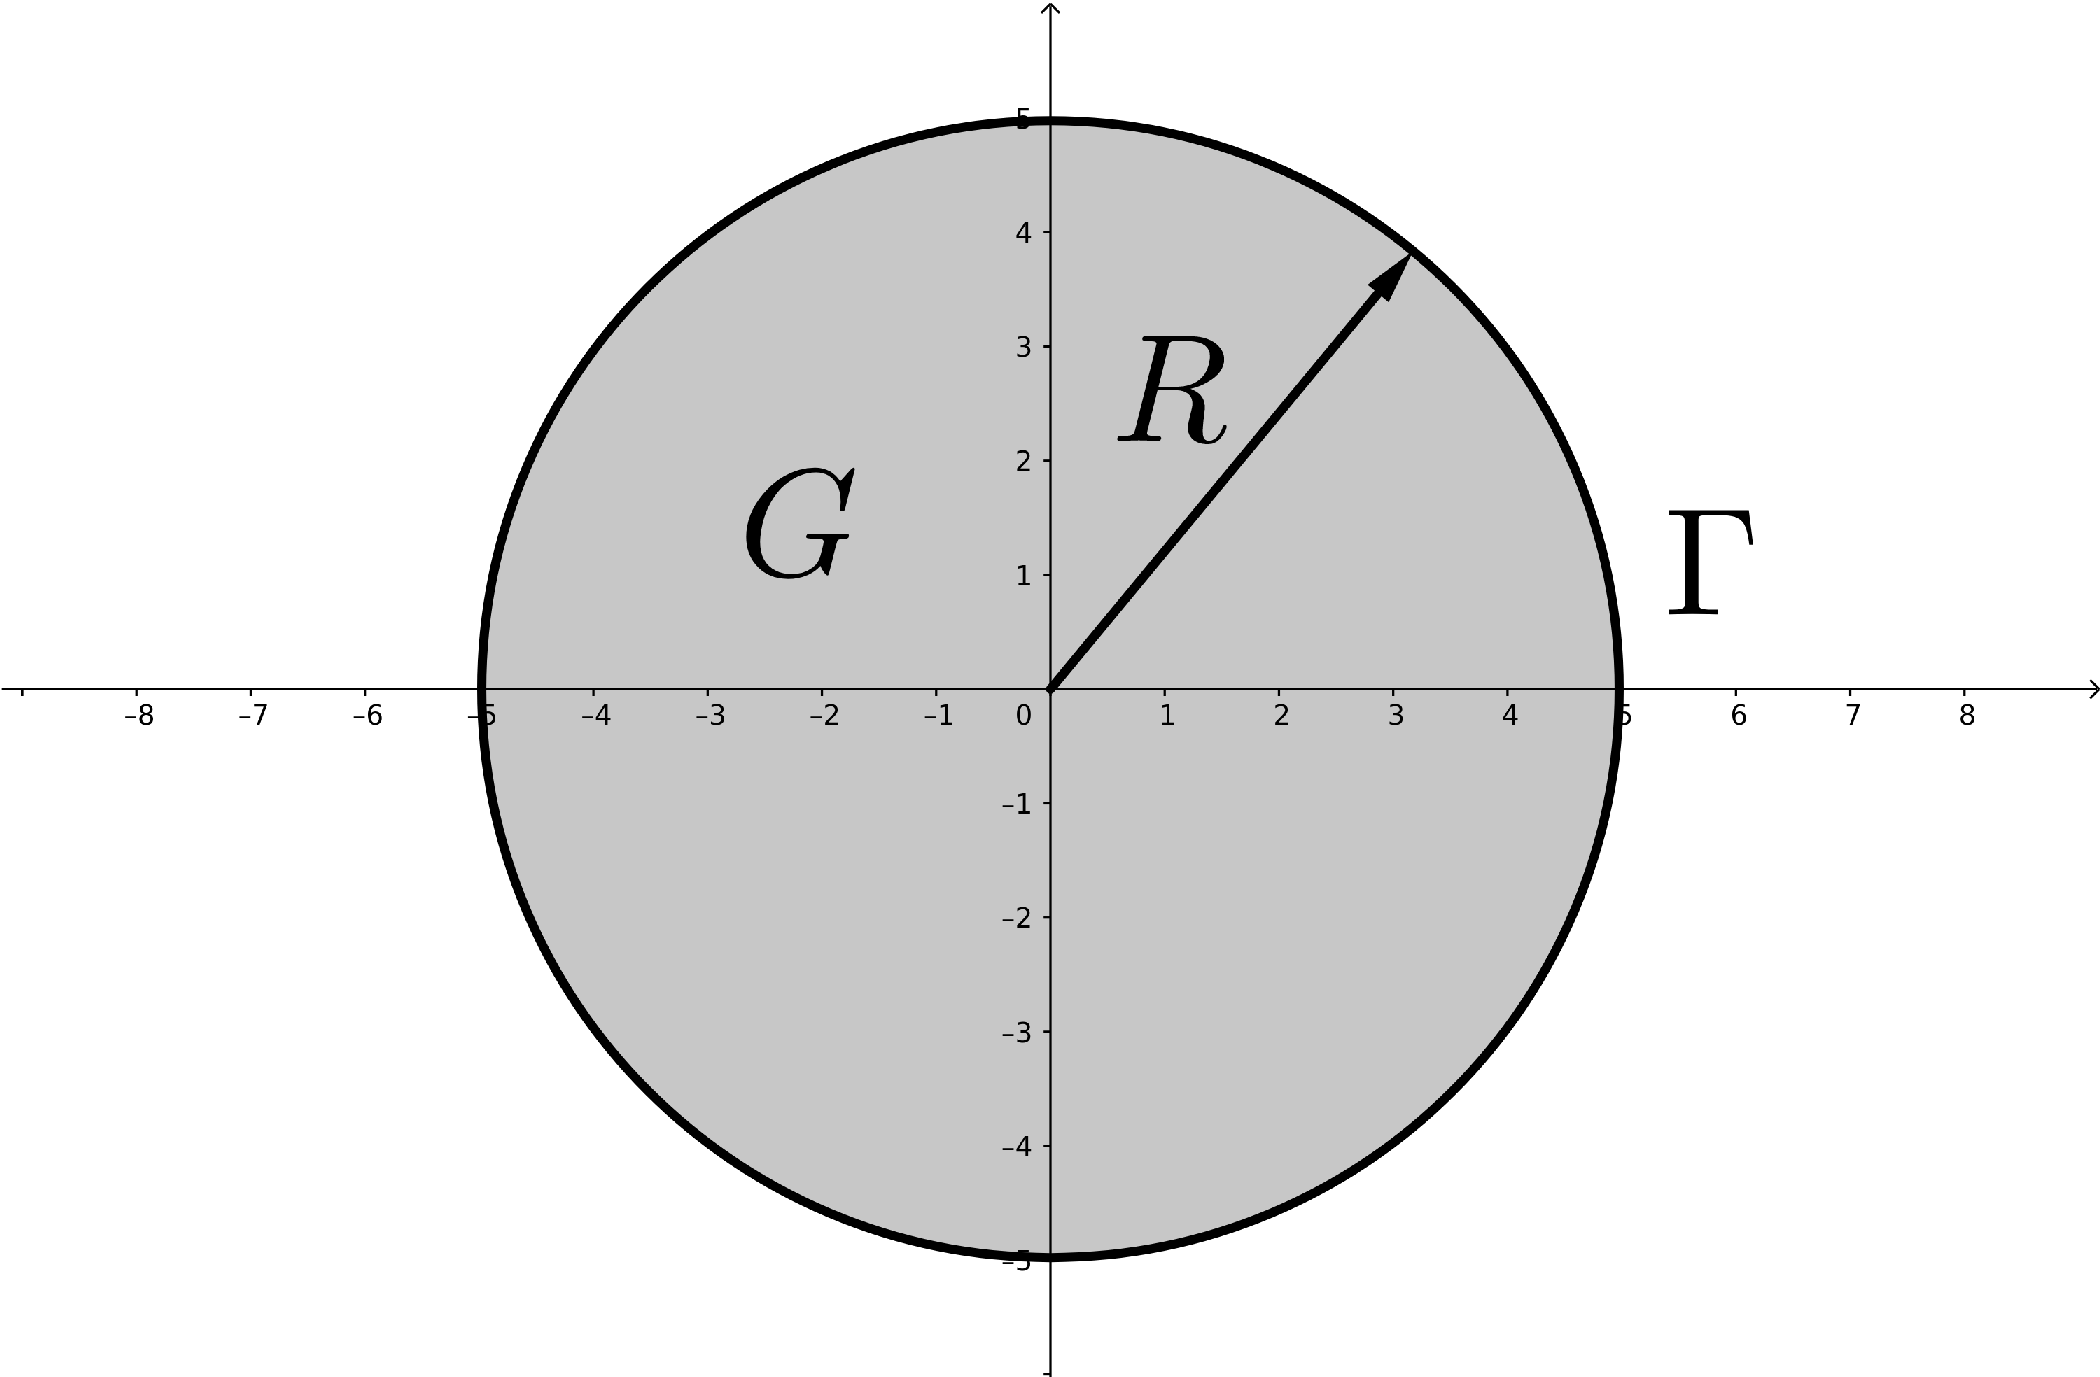
\includegraphics[scale=0.1]{laplacecircle.png} 
\end{center}
\[
    G = \left\lbrace (x,y):x^2+y^2 < R^2 \right\rbrace  \;\;\;\;\;\;\;\;\;\ \Gamma = \left\lbrace (x,y):x^2+y^2 = R^2 \right\rbrace    
\]
Equations involving such conditions are classified as Drichlet problems.
%%%%%%%%%%%%%%%%%%%%%%%%%%%%%%%%%%%%%%%%%%
%%%%%%%%%%%%%%%%%%%%%%%%%%%%%%%%%%%%%%%%%%
%%%%%%%%%%%%%%%%%%%%%%%%%%%%%%%%%%%%%%%%%%
%%%%%%%%%%%%%%%%%%%%%%%%%%%%%%%%%%%%%%%%%%
%%%%%%%%%%%%%%%%%%%%%%%%%%%%%%%%%%%%%%%%%%
\subsection*{Intial Condition}
The initial condition is a condition that a solution must have at only on instant of time, which is the starting time as it can be found expremintally. An example is the heat equation with intial condition.
\begin{align*}
\frac{\partial u(x,t)}{\partial t}  &= c^2 \frac{\partial u(x,t)}{\partial x}
\\
\\
u(x,0) &= f(x)
\end{align*}
Equations involving such conditions are classified as Cauchy problems.
\subsection*{Equations of Mathematical Physics}
The most frequently incountered equations in physics are the following
\begin{enumerate}
\item Heat Equation
\begin{align*}
\frac{\partial u(x,t)}{\partial t}  &= c^2 \frac{\partial^2 u(x,t)}{\partial x^2}
\end{align*}

\item Wave Equation 
\begin{align*}
\frac{\partial^2 u(x,t)}{\partial t^2}  &= c^2 \frac{\partial^2 u(x,t)}{\partial x^2}
\end{align*}

\item Laplace's Equation
\begin{align*}
\nabla^2 u(x) = \frac{\partial^2 u(x)}{\partial x^{2}_{1}} + \frac{\partial^2 u(x)}{\partial x^{2}_{2}} + \frac{\partial^2 u(x)}{\partial x^{2}_{3}} + \cdots = 0
\end{align*}
\end{enumerate}

those will be our main focus in this course.
\\

\end{document}